% This work is licensed under the Creative Commons
% Attribution-NonCommercial-ShareAlike 4.0 International License. To view a copy
% of this license, visit http://creativecommons.org/licenses/by-nc-sa/4.0/ or
% send a letter to Creative Commons, PO Box 1866, Mountain View, CA 94042, USA.

\section{Einführung in algebraische Modellierung}

Die \define{Strukturmathematik} stellt sich die Aufgabe Strukturen zu modellieren und technisch wie sprachlich zugänglich zu machen, sogenannte \define{Theoriebildung}.
Dies ist ein evolutionärer Prozess, in dem neue Begriffe entstehen und alte untergehen.

\subsection{Warum Modellierung und Formalisierung?}

\begin{figure}[H]
	\begin{center}
		% This work is licensed under the Creative Commons
% Attribution-NonCommercial-ShareAlike 4.0 International License. To view a copy
% of this license, visit http://creativecommons.org/licenses/by-nc-sa/4.0/ or
% send a letter to Creative Commons, PO Box 1866, Mountain View, CA 94042, USA.

\tikzset{every picture/.style={line width=0.75pt}} %set default line width to 0.75pt        

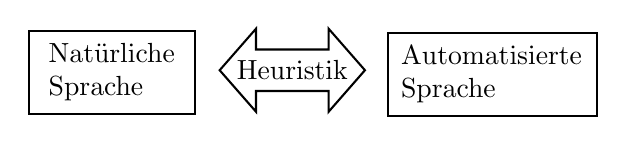
\begin{tikzpicture}[x=0.75pt,y=0.75pt,yscale=-1,xscale=1]
%uncomment if require: \path (0,300); %set diagram left start at 0, and has height of 300

%Shape: Rectangle [id:dp02241090211127661] 
\draw   (81,126) -- (161,126) -- (161,166) -- (81,166) -- cycle ;
%Shape: Rectangle [id:dp20165869726734287] 
\draw   (254,127) -- (355,127) -- (355,167) -- (254,167) -- cycle ;
%Left Right Arrow [id:dp33351638469477385] 
\draw   (173,145) -- (190.5,125) -- (190.5,135) -- (225.5,135) -- (225.5,125) -- (243,145) -- (225.5,165) -- (225.5,155) -- (190.5,155) -- (190.5,165) -- cycle ;

% Text Node
\draw (121,146) node  [align=left] {Natürliche\\Sprache};
% Text Node
\draw (304,147) node  [align=left] {Automatisierte\\Sprache};
% Text Node
\draw (208,145) node  [align=left] {Heuristik};


\end{tikzpicture}
		%\caption{Modellierung}
		%\label{Abb:natSpracheModellierung}
	\end{center}
\end{figure}

\betone{Problem:} Fehlkommunikation\\
Das fehlende Glied ist die Formale Sprache:

\begin{figure}[H] % oder ht!
	\begin{center}
		% This work is licensed under the Creative Commons
% Attribution-NonCommercial-ShareAlike 4.0 International License. To view a copy
% of this license, visit http://creativecommons.org/licenses/by-nc-sa/4.0/ or
% send a letter to Creative Commons, PO Box 1866, Mountain View, CA 94042, USA.

\tikzset{every picture/.style={line width=0.75pt}} %set default line width to 0.75pt        

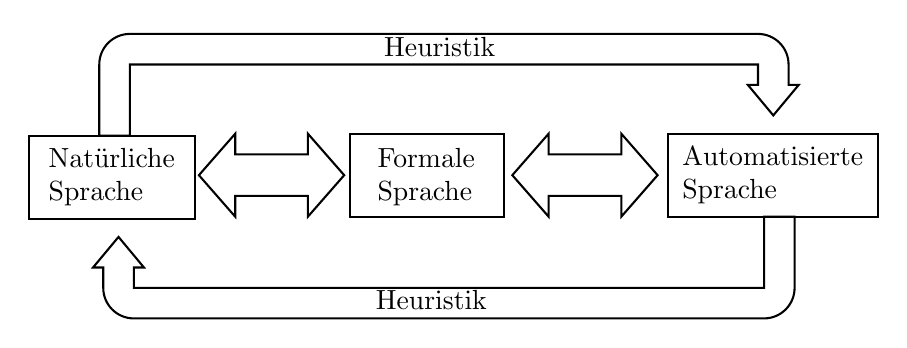
\begin{tikzpicture}[x=0.75pt,y=0.75pt,yscale=-1,xscale=1]
%uncomment if require: \path (0,300); %set diagram left start at 0, and has height of 300

%Shape: Rectangle [id:dp02241090211127661] 
\draw   (81,126) -- (161,126) -- (161,166) -- (81,166) -- cycle ;
%Shape: Rectangle [id:dp20165869726734287] 
\draw   (236,125) -- (310,125) -- (310,165) -- (236,165) -- cycle ;
%Left Right Arrow [id:dp33351638469477385] 
\draw   (163,145) -- (180.5,125) -- (180.5,135) -- (215.5,135) -- (215.5,125) -- (233,145) -- (215.5,165) -- (215.5,155) -- (180.5,155) -- (180.5,165) -- cycle ;
%Shape: Rectangle [id:dp2972974344682269] 
\draw   (389,125) -- (490,125) -- (490,165) -- (389,165) -- cycle ;
%Left Right Arrow [id:dp8197742277124606] 
\draw   (314,145) -- (331.5,125) -- (331.5,135) -- (366.5,135) -- (366.5,125) -- (384,145) -- (366.5,165) -- (366.5,155) -- (331.5,155) -- (331.5,165) -- cycle ;
%U Turn Arrow [id:dp49299810652548426] 
\draw   (115,126) -- (115,91.65) .. controls (115,83.52) and (121.59,76.93) .. (129.72,76.93) -- (432.37,76.93) .. controls (440.5,76.93) and (447.09,83.52) .. (447.09,91.65) -- (447.09,101.47) -- (452,101.47) -- (439.73,116.19) -- (427.47,101.47) -- (432.37,101.47) -- (432.37,91.65) .. controls (432.37,91.65) and (432.37,91.65) .. (432.37,91.65) -- (129.72,91.65) .. controls (129.72,91.65) and (129.72,91.65) .. (129.72,91.65) -- (129.72,126) -- cycle ;
%U Turn Arrow [id:dp46223682559547996] 
\draw   (450,164.93) -- (450,199.28) .. controls (450,207.41) and (443.41,214) .. (435.28,214) -- (131.63,214) .. controls (123.5,214) and (116.91,207.41) .. (116.91,199.28) -- (116.91,189.47) -- (112,189.47) -- (124.27,174.75) -- (136.53,189.47) -- (131.63,189.47) -- (131.63,199.28) .. controls (131.63,199.28) and (131.63,199.28) .. (131.63,199.28) -- (435.28,199.28) .. controls (435.28,199.28) and (435.28,199.28) .. (435.28,199.28) -- (435.28,164.93) -- cycle ;

% Text Node
\draw (121,146) node  [align=left] {Natürliche\\Sprache};
% Text Node
\draw (439.5,145) node  [align=left] {Automatisierte\\Sprache};
% Text Node
\draw (272.5,146) node  [align=left] {Formale\\Sprache};
% Text Node
\draw (279,83) node  [align=left] {Heuristik};
% Text Node
\draw (275,205) node  [align=left] {Heuristik};


\end{tikzpicture}

		%\caption{Modellierung}
		%\label{Abb:natSpracheModellierung}
	\end{center}
\end{figure}

Die Formale Sprache erlaubt Absraktion und Vergleich.
Die automatisierte Sprache ist algorithmisch reichhaltig, aber strukturell arm.
Im Sinne der mathematischen Beschreibung / Modellierung ist ein Modell-Vergleich oft nicht möglich, wenn ich kein abstraktes Modell habe!\nl
Es gibt zwei Wege, Wissen zu erlangen:
\begin{enumerate}
	\item \define{Top Down:} deduktive Methode (allgemeine Aussage $\to$ Einzelfall)
	\item \define{Bottom Up:} induktive Methode (Einzelfall $\to$ allgemeine Aussage)
\end{enumerate}

\define{Technische Makros} sind symbolische Abkürzungen, z.B. "$\R$".
Im Gegensatz dazu gibt es auch \define{verbale Makros}, z.B. "reelle Zahlen".
\index{technisches Makro}
\index{verbales Makro}

\subsection{Mengenbasierte Modellierung / strukturelle Modellierung}

Strukturelle Modellierung ist eine mengenbasierte Modellierung.
Dies ist ein Gegensatz z.B. zur \textbf{Prozedurale Modellierung}.

\section{\href{https://de.wikipedia.org/wiki/Inzidenzstruktur}{Inzidenzstrukturen}}
\begin{definition}
	Seien $P,B$ disjunkte Mengen und sei $I\subseteq P\times B$.
	Dann heißt das Tripel $\Inz=(P,B,I)$ \define{Inzidenzstruktur}.
	\index{Inzidenzstruktur}
	\begin{itemize}
		\item Elemente von $P$ heißen \define{Punkten / Points}.
		\item Elemente von $B$ heißen \define{Blöcke / Blocks}.
		\item $I$ heißt \define{Inzidenzrelation} und die Elemente von $I$ heißen \define{Inzidenzen / Fahnen}.
	\end{itemize}
	Wir schreiben auch
	\begin{align*}
		pIb\defiff (p,b)\in I
	\end{align*}
	und sagen dazu:
	"Der Punkt $p$ inzidiert mit dem Block $b$ in $\Inz$."\\
	Für $p\in P$ sei
	\begin{align*}
		pI:=\set{b\in B\mid pIb}
	\end{align*}
	d.h. die Menge aller mit dem Punkt $p$ inzidierenden Blöcke.\\
	Analog sei für $b\in B$ stets
	\begin{align*}
		Ib:=\set{p\in P\mid pIb}
	\end{align*}
	die Menge aller mit dem Block $b$ inzidierenden Punkte.
\end{definition}

\begin{beispiel}\
	\begin{itemize}
		\item $P:=$ Eckenmenge eines Würfels
		\item $B:=$ Flächenmenge des Würfels
		\item Inzidenz: Punkt ist Eckpunkt von Würfelfläche
	\end{itemize}
\end{beispiel}

\begin{definition}
	Eine Inzidenzstruktur $\Inz=(P,B,I)$ heißt \define{endlich}
	\begin{align*}
		\defiff \#P,\#B<\infty
	\end{align*}
	Hierbei bezeichnet $\#M$ die Anzahl der Elemente der Menge $M$.
\end{definition}

\begin{satz}[Prinzip der doppelten Abzählung]\label{satzDoppelteAbzahlung}\enter
	Für jede endliche Inzidenzstrukut $\Inz=(P,B,I)$ gilt:
	\begin{align*}
		\sum\limits_{p\in P}\# pI=\#I=\sum\limits_{b\in B}\# Ib
	\end{align*}
\end{satz}

\begin{definition}
	$\Inz=(P,B,I)$ heißt \define{\href{https://de.wikipedia.org/wiki/Taktische_Zerlegung}{taktische Konfiguration}}
	\index{taktische Konfiguration} 
	\begin{align*}
		\defiff\exists r_\Inz,k_\Inz\in\N:\forall p\in P,\forall b\in B:\# pI=r_\Inz\und\#Ib=k_\Inz
	\end{align*}
\end{definition}

\begin{lemma}
	Für jede taktische Konfiguration $\Inz=(P,B,I)$ gilt:
	\begin{align*}
		v_\Inz\mal r_\Inz=b_\Inz\mal k_\Inz
		\qquad\mit\qquad
		v_\Inz:=\# P\und b_\Inz:=\#B
	\end{align*}
\end{lemma}

\begin{proof}
	Folgt aus Satz \ref{satzDoppelteAbzahlung}:
	\begin{align*}
		v_\Inz\mal r_\Inz=\sum\limits_{p\in P}\underbrace{\# pI}_{=r_\Inz}=\sum\limits_{b\in B}\underbrace{\#Ib}_{=k_\Inz}=b_\Inz\mal r_\Inz
	\end{align*}
\end{proof}

\begin{definition}
	$\big(v_\Inz,r_\Inz;b_\Inz,k_\Inz)$ ist das \define{Parametertupel} von $\Inz$.
	\index{Parametertupel}\index{duales Parametertupel}\\
	Das dazu \define{duale Parametertupel} ist $\big(b_\Inz,k_\Inz;v_\Inz,r_\Inz\big)$.
\end{definition}

\begin{beispiel}
	Für unsere Würfelinzidenzstruktur ist das Parametertupel:\\
	(Anzahl der Punkte, Anzahl der Geraden pro Punkt, Anzahl der Geraden, Anzahl der Punkte pro Gerade).
	\begin{enumerate}
		\item Tetraeder (dual Tetraeder): $(4,3;4,3)$ 
		\item Hexader (dual: Oktaeder): $(8,3;6,4)$
		\item Dodekaeder (dual: Ikosaeder): $(20,3;12,5)$
		\item Dreieck: $(3,2;3,2)$ ist auch selbstdual: Dreieck $\leftrightarrow$ Dreiseit
	\end{enumerate}
\end{beispiel}

\begin{beispiel}[Veblen-Young-Configuration]\
	\begin{figure}[H] % oder ht!
		\begin{center}
			% This work is licensed under the Creative Commons
% Attribution-NonCommercial-ShareAlike 4.0 International License. To view a copy
% of this license, visit http://creativecommons.org/licenses/by-nc-sa/4.0/ or
% send a letter to Creative Commons, PO Box 1866, Mountain View, CA 94042, USA.



\tikzset{every picture/.style={line width=0.75pt}} %set default line width to 0.75pt        

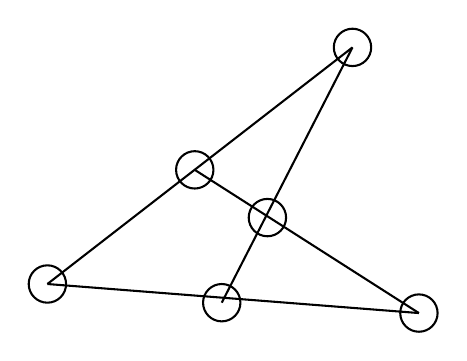
\begin{tikzpicture}[x=0.75pt,y=0.75pt,yscale=-1,xscale=1]
%uncomment if require: \path (0,300); %set diagram left start at 0, and has height of 300

%Shape: Circle [id:dp8256548323361356] 
\draw   (15,144) .. controls (15,139.03) and (19.03,135) .. (24,135) .. controls (28.97,135) and (33,139.03) .. (33,144) .. controls (33,148.97) and (28.97,153) .. (24,153) .. controls (19.03,153) and (15,148.97) .. (15,144) -- cycle ;
%Shape: Circle [id:dp9999136902725693] 
\draw   (162,30) .. controls (162,25.03) and (166.03,21) .. (171,21) .. controls (175.97,21) and (180,25.03) .. (180,30) .. controls (180,34.97) and (175.97,39) .. (171,39) .. controls (166.03,39) and (162,34.97) .. (162,30) -- cycle ;
%Shape: Circle [id:dp7722874472312242] 
\draw   (86,89) .. controls (86,84.03) and (90.03,80) .. (95,80) .. controls (99.97,80) and (104,84.03) .. (104,89) .. controls (104,93.97) and (99.97,98) .. (95,98) .. controls (90.03,98) and (86,93.97) .. (86,89) -- cycle ;
%Shape: Circle [id:dp1591555646648798] 
\draw   (194,158) .. controls (194,153.03) and (198.03,149) .. (203,149) .. controls (207.97,149) and (212,153.03) .. (212,158) .. controls (212,162.97) and (207.97,167) .. (203,167) .. controls (198.03,167) and (194,162.97) .. (194,158) -- cycle ;
%Shape: Circle [id:dp04988684193722637] 
\draw   (121,112) .. controls (121,107.03) and (125.03,103) .. (130,103) .. controls (134.97,103) and (139,107.03) .. (139,112) .. controls (139,116.97) and (134.97,121) .. (130,121) .. controls (125.03,121) and (121,116.97) .. (121,112) -- cycle ;
%Shape: Circle [id:dp15540025125472967] 
\draw   (99,153) .. controls (99,148.03) and (103.03,144) .. (108,144) .. controls (112.97,144) and (117,148.03) .. (117,153) .. controls (117,157.97) and (112.97,162) .. (108,162) .. controls (103.03,162) and (99,157.97) .. (99,153) -- cycle ;
%Straight Lines [id:da9051529769910057] 
\draw    (24,144) -- (171,30) ;


%Straight Lines [id:da9722531504709364] 
\draw    (24,144) -- (203,158) ;


%Straight Lines [id:da879150422612323] 
\draw    (95,89) -- (203,158) ;


%Straight Lines [id:da809884536800273] 
\draw    (171,30) -- (108,153) ;

\end{tikzpicture}

			\caption{Veblen-Young-Konfiguration: $(6,2;4,3)$}
			%\label{Abb:natSpracheModellierung}
		\end{center}
	\end{figure}
	\begin{figure}[H] % oder ht!
		\begin{center}
			% This work is licensed under the Creative Commons
% Attribution-NonCommercial-ShareAlike 4.0 International License. To view a copy
% of this license, visit http://creativecommons.org/licenses/by-nc-sa/4.0/ or
% send a letter to Creative Commons, PO Box 1866, Mountain View, CA 94042, USA.


\tikzset{every picture/.style={line width=0.75pt}} %set default line width to 0.75pt        

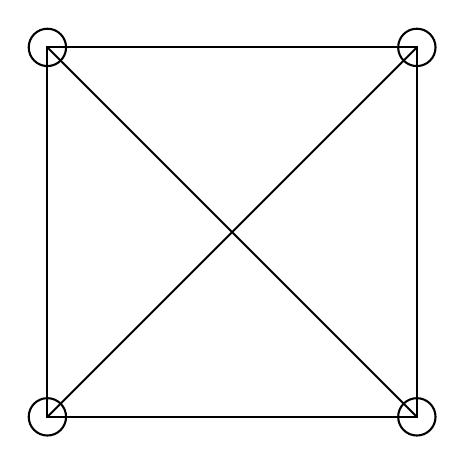
\begin{tikzpicture}[x=0.75pt,y=0.75pt,yscale=-1,xscale=1]
%uncomment if require: \path (0,300); %set diagram left start at 0, and has height of 300

%Shape: Square [id:dp9706132534648327] 
\draw   (201,62) -- (379,62) -- (379,240) -- (201,240) -- cycle ;
%Straight Lines [id:da9618724140233941] 
\draw    (201,62) -- (379,240) ;


%Straight Lines [id:da3907949926394131] 
\draw    (379,62) -- (201,240) ;


%Shape: Circle [id:dp5133007782867983] 
\draw   (192,62) .. controls (192,57.03) and (196.03,53) .. (201,53) .. controls (205.97,53) and (210,57.03) .. (210,62) .. controls (210,66.97) and (205.97,71) .. (201,71) .. controls (196.03,71) and (192,66.97) .. (192,62) -- cycle ;
%Shape: Circle [id:dp3477876429055702] 
\draw   (192,240) .. controls (192,235.03) and (196.03,231) .. (201,231) .. controls (205.97,231) and (210,235.03) .. (210,240) .. controls (210,244.97) and (205.97,249) .. (201,249) .. controls (196.03,249) and (192,244.97) .. (192,240) -- cycle ;
%Shape: Circle [id:dp36747093980837164] 
\draw   (370,240) .. controls (370,235.03) and (374.03,231) .. (379,231) .. controls (383.97,231) and (388,235.03) .. (388,240) .. controls (388,244.97) and (383.97,249) .. (379,249) .. controls (374.03,249) and (370,244.97) .. (370,240) -- cycle ;
%Shape: Circle [id:dp00705377401053342] 
\draw   (370,62) .. controls (370,57.03) and (374.03,53) .. (379,53) .. controls (383.97,53) and (388,57.03) .. (388,62) .. controls (388,66.97) and (383.97,71) .. (379,71) .. controls (374.03,71) and (370,66.97) .. (370,62) -- cycle ;

\end{tikzpicture}

			\caption{duale Veblen-Young-Konfiguration: $(4,3;6,2)$}
			%\label{Abb:natSpracheModellierung}
		\end{center}
	\end{figure}	
\end{beispiel}

\begin{beispiel}\label{beispInzidenz}
	Berühmte taktische Konfiguation ist $(10,3;10,3)$.\\
	Sei $[n]:=\set{1,\ldots,n}$ für $n\in\N$ und $\ul{n}:=\set{0,\ldots,n-1}$.
	Sei $\begin{pmatrix}
		M\\k
	\end{pmatrix}:=\set{X\subseteq M\mid\#X=k}$ für $M$ Menge.
	Dann gilt $\#\begin{pmatrix}
		M\\k
	\end{pmatrix}=\begin{pmatrix}
		\#M\\k
	\end{pmatrix}$.
	Seien $i,j,n\in\N$ mit $i\leq j\leq n$.
	Setze
	\begin{align*}
		\Inz^n_{(i,j)}&:=\klammern{\begin{pmatrix}
			[n]\\i
		\end{pmatrix},\begin{pmatrix}
			[n]\\ j
		\end{pmatrix},I^n_{(i,j)}}\qquad\mit\\
		I^n_{(i,j)}&:=\set{(p,b)\in\begin{pmatrix}
			[n]\\ i
		\end{pmatrix}\times\begin{pmatrix}
			[n]\\j
		\end{pmatrix}\mid p\subseteq b}
	\end{align*}
	Dann ist $\Inz^n_{(i,j)}$ taktische Konfiguration mit dem Parametertupel
	\begin{align*}
		\klammern{
		\begin{pmatrix}
			n\\i
		\end{pmatrix},
		\begin{pmatrix}
			n-i\\j-i
		\end{pmatrix},
		\begin{pmatrix}
			n\\j
		\end{pmatrix},
		\begin{pmatrix}
			j\\i
		\end{pmatrix}
		}
	\end{align*}
	Wann ist dies gleich $(10,3;10,3)$?
	Oder gleich $(4,3;6,2)$? Antwort:
	\begin{align*}
		(4,3;6,2)=\klammern{\begin{pmatrix}
			4\\1
		\end{pmatrix},\begin{pmatrix}
			4-1\\2-1
		\end{pmatrix},
		\begin{pmatrix}
			4\\2
		\end{pmatrix},
		\begin{pmatrix}
			2\\1
		\end{pmatrix}}
	\end{align*}
	dh. $(i,j,n)=(1,2,4)$.
\end{beispiel}

\begin{definition}
	Die \define{duale Inzidenzstruktur} einer Inzidenzstruktur $\Inz=(P,B,I)$ ist
	\index{duale Inzidenzstruktur}
	\begin{align*}
		\Inz^{\op}:=\big(B,P,I^\op\big)
		\qquad\mit\qquad
		I^\op:=\set{(b,p)\in B\times P\mid p I b}
	\end{align*}
\end{definition}

\begin{beispiel}[Fortsetzung von Beispiel \ref{beispInzidenz}]
	\begin{align*}
		\Big(\Inz_{(i,j)}^n\Big)^\op=(B,P,R^\op)
		\qquad\mit\qquad
		R^\op:=\set{(b,p)\in\begin{pmatrix}
			[n]\\
			j
		\end{pmatrix}\times
		\begin{pmatrix}
			[n]\\
			i
		\end{pmatrix}:p\subseteq b}
	\end{align*}
\end{beispiel}

\begin{definition}
	Seien $\Inz=(P,B,I)$ und $\Inz'=(P',B',I')$ Inzidenzstrukturen.
	Dann heißt ein Abbildungspaar $(\varphi,\psi)$ bestehend aus Abbildungen $\varphi\colon P\to P'$ und $\psi\colon B\to B'$ ein \define{Morphismus} von $\Inz$ nach $\Inz'$
	\index{Morphismus}\index{Isomorphismus}
	\begin{align*}
		\defiff\forall p\in P,\forall b\in B:pIb\implies\varphi(p)I'\psi(b)
	\end{align*}

	Ein Abbildungspaar $(\varphi,\psi)$ bestehend aus Bijektionen $\varphi\colon P\to P'$ und $\psi\colon B\to B'$ heißt \define{Isomorphismus (Iso)} von $\Inz$ nach $\Inz'$
	\begin{align*}
		\defiff\forall p\in P,\forall b\in B:pIb\iff\varphi(p)I'\psi(b)
\end{align*}		
	
	Wir sagen, $\Inz$ ist \define{isomorph} zu $\Inz'$, i.Z. $\Inz\simeq\Inz'$, falls es einen Isomorphismus von $\Inz$ nach $\Inz'$ gibt.
\end{definition}

\begin{lemma}\
	\begin{enumerate}
		\item Ist $(\varphi,\psi)$ ein Isomorphismus von $\Inz$ nach $\Inz'$, so ist auch $\big(\varphi^{-1},\psi^{-1}\big)$ ein Isomorphismus von $\Inz'$ nach $\Inz$.\label{item:lemma1.13_1}
		\item Ist $(\varphi,\psi)$ Morphismus von $\Inz$ nach $\Inz'$, so ist $(\psi,\varphi)$ Morphismus von $\Inz^\op$ nach $(\Inz')^\op$.\label{item:lemma1.13_2}
	\end{enumerate}
\end{lemma}

\begin{proof}
	\betone{Zeige \ref{item:lemma1.13_1}:}\\
	Seien $p'\in P'$ und $b'\in B'$ mit $p'I'b'$.
	Zu zeigen ist
	\begin{align*}
		\varphi^{-1}(b')=\psi^{-1}(b')
	\end{align*}
	Wegen $p'I'b'$ gilt für $p:=\varphi^{-1}(p')$ und $b:=\psi^{-1}(b')$ stets $\varphi(p)=p'$ und $sp(b)=b'$, also $\varphi(p)I'\psi(b)$.
	Also gilt auch $pIb$ d.h. $\varphi^{-1}(p)I\psi^{-1}(b)$.\nl
	\betone{Zeige \ref{item:lemma1.13_2}:} Total klar.
\end{proof}

\begin{satz}
	Seien $i,j,n\in\N$ mit $i\leq j\leq n$.
	Dann gilt
	\begin{align*}
		\Big(\Inz_{(i,j)}^n\Big)^\op\simeq\Inz_{(n-j,n-i)}^n
	\end{align*}
	vermöge $(\varphi,\psi)$ mit
	\begin{align*}
		\varphi\colon		
		\underbrace{
		\begin{pmatrix}
			[n]\\
			j
		\end{pmatrix}}_{
		\text{Punktmenge von }\big(\Inz_{(i,j)}^n\big)^\op
		}&\to\underbrace{\begin{pmatrix}
			[n]\\
			n-j
		\end{pmatrix}}_{
		\text{Punktmenge von }\Inz_{(n-j,n-i)}^n
		}
		&&
		b\mapsto[n]-b\\
	\psi\colon\underbrace{\begin{pmatrix}
			[n]\\
			i
		\end{pmatrix}}_{
		\text{Blockmenge von }\big(\Inz_{(i,j)}^n\big)^\op
		}&\to\underbrace{\begin{pmatrix}
			[n]\\
			n-i
		\end{pmatrix}}_{
		\text{Blockmenge von }\Inz_{(n-j,n-i)}^n
		}
		&&
		p\mapsto[n]-p
	\end{align*}
	Also sind die Parametertupel von $\Big(\Inz_{(i,j)}^n\Big)^\op$ gegeben durch
	\begin{align*}
		\klammern{
		\begin{pmatrix}
			n\\
			j
		\end{pmatrix},
		\begin{pmatrix}
			n-i\\
			j-i
		\end{pmatrix};
		\begin{pmatrix}
			n\\
			i
		\end{pmatrix},
		\begin{pmatrix}
			j\\ 
			i
		\end{pmatrix}}
	\end{align*}
	und von $\Inz_{(n-j,n-i)}^n$ gegeben durch
	\begin{align*}
		\klammern{
		\begin{pmatrix}
			n\\
			n-j
		\end{pmatrix},
		\begin{pmatrix}
			n-(n-j)\\
			(n-i)-(n-j)
		\end{pmatrix},
		\begin{pmatrix}
			n\\
			n-i
		\end{pmatrix},
		\begin{pmatrix}
			n-i\\
			n-j
		\end{pmatrix}}
	\end{align*}
	gleich.
\end{satz}

\begin{definition}
	Eine Inzidenzstruktur $\Inz$ heißt \define{selbstdual}\index{selbstdual}
	\begin{align*}
		\defiff\Inz\simeq\Inz^\op
	\end{align*}
\end{definition}

Wann ist $\Inz_{(i,j)}^n$ selbstdual?

\begin{lemma}
	Für $0<i\leq j\leq n$ gilt:
	\begin{align*}
		\Inz_{(i,j)}^n\simeq\Inz_{(i',j')}^{n'}\iff
		(i,j,n)=(i',j',n')
	\end{align*}
\end{lemma}

\begin{satz}
	\begin{align*}
		\Inz_{(i,j)}^n\text{ selbstdual}
		&\iff \Inz_{(i,j)}^n\simeq\Big(\Inz_{(i,j)}^n\Big)^\op\simeq \Inz_{(n-j,n-i)}^n\\
		&\iff i=n-j\und j=n-i\\
		&\iff i+j=n
	\end{align*}
\end{satz}

\begin{beispiel}
	Für welches Tripel $(i,j,n)$ hat die Inzidenzstruktur $\Inz_{(i,j)}^n$ das Parametertupel $(10,3;10,3)$?\\
	Antwort: für $(i,j,n)=(2,3,5)$.
	Geometrische Realisierung von $\Inz_{(2,3)}^5$:
	\begin{figure}[H] % oder ht!
		\begin{center}
			% This work is licensed under the Creative Commons
% Attribution-NonCommercial-ShareAlike 4.0 International License. To view a copy
% of this license, visit http://creativecommons.org/licenses/by-nc-sa/4.0/ or
% send a letter to Creative Commons, PO Box 1866, Mountain View, CA 94042, USA.




\tikzset{every picture/.style={line width=0.75pt}} %set default line width to 0.75pt        

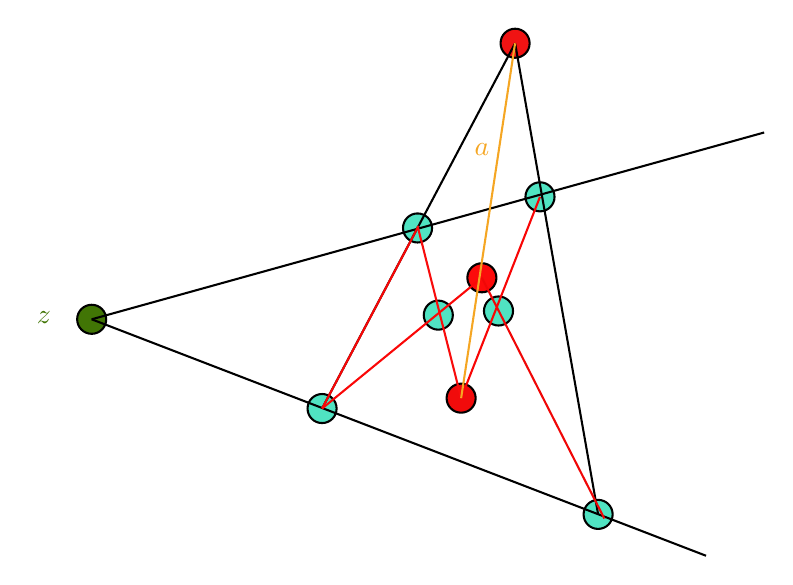
\begin{tikzpicture}[x=0.75pt,y=0.75pt,yscale=-1,xscale=1]
%uncomment if require: \path (0,300); %set diagram left start at 0, and has height of 300

%Shape: Circle [id:dp08312604554148328] 
\draw  [fill={rgb, 255:red, 80; green, 227; blue, 194 }  ,fill opacity=1 ] (192,142) .. controls (192,138.13) and (195.13,135) .. (199,135) .. controls (202.87,135) and (206,138.13) .. (206,142) .. controls (206,145.87) and (202.87,149) .. (199,149) .. controls (195.13,149) and (192,145.87) .. (192,142) -- cycle ;
%Shape: Circle [id:dp5479371678347926] 
\draw  [fill={rgb, 255:red, 80; green, 227; blue, 194 }  ,fill opacity=1 ] (182,100) .. controls (182,96.13) and (185.13,93) .. (189,93) .. controls (192.87,93) and (196,96.13) .. (196,100) .. controls (196,103.87) and (192.87,107) .. (189,107) .. controls (185.13,107) and (182,103.87) .. (182,100) -- cycle ;
%Shape: Circle [id:dp9035059763139627] 
\draw  [fill={rgb, 255:red, 241; green, 11; blue, 11 }  ,fill opacity=1 ] (203,182) .. controls (203,178.13) and (206.13,175) .. (210,175) .. controls (213.87,175) and (217,178.13) .. (217,182) .. controls (217,185.87) and (213.87,189) .. (210,189) .. controls (206.13,189) and (203,185.87) .. (203,182) -- cycle ;
%Shape: Circle [id:dp13405737177609034] 
\draw  [fill={rgb, 255:red, 65; green, 117; blue, 5 }  ,fill opacity=1 ] (25,144) .. controls (25,140.13) and (28.13,137) .. (32,137) .. controls (35.87,137) and (39,140.13) .. (39,144) .. controls (39,147.87) and (35.87,151) .. (32,151) .. controls (28.13,151) and (25,147.87) .. (25,144) -- cycle ;
%Shape: Circle [id:dp820938089239013] 
\draw  [fill={rgb, 255:red, 240; green, 19; blue, 19 }  ,fill opacity=1 ] (229,11) .. controls (229,7.13) and (232.13,4) .. (236,4) .. controls (239.87,4) and (243,7.13) .. (243,11) .. controls (243,14.87) and (239.87,18) .. (236,18) .. controls (232.13,18) and (229,14.87) .. (229,11) -- cycle ;
%Shape: Circle [id:dp9814130832419268] 
\draw  [fill={rgb, 255:red, 80; green, 227; blue, 194 }  ,fill opacity=1 ] (136,187) .. controls (136,183.13) and (139.13,180) .. (143,180) .. controls (146.87,180) and (150,183.13) .. (150,187) .. controls (150,190.87) and (146.87,194) .. (143,194) .. controls (139.13,194) and (136,190.87) .. (136,187) -- cycle ;
%Shape: Circle [id:dp7483452900473003] 
\draw  [fill={rgb, 255:red, 80; green, 227; blue, 194 }  ,fill opacity=1 ] (241,85) .. controls (241,81.13) and (244.13,78) .. (248,78) .. controls (251.87,78) and (255,81.13) .. (255,85) .. controls (255,88.87) and (251.87,92) .. (248,92) .. controls (244.13,92) and (241,88.87) .. (241,85) -- cycle ;
%Shape: Circle [id:dp47277380471474084] 
\draw  [fill={rgb, 255:red, 80; green, 227; blue, 194 }  ,fill opacity=1 ] (269,238) .. controls (269,234.13) and (272.13,231) .. (276,231) .. controls (279.87,231) and (283,234.13) .. (283,238) .. controls (283,241.87) and (279.87,245) .. (276,245) .. controls (272.13,245) and (269,241.87) .. (269,238) -- cycle ;
%Shape: Circle [id:dp9584244691590221] 
\draw  [fill={rgb, 255:red, 80; green, 227; blue, 194 }  ,fill opacity=1 ] (221,140) .. controls (221,136.13) and (224.13,133) .. (228,133) .. controls (231.87,133) and (235,136.13) .. (235,140) .. controls (235,143.87) and (231.87,147) .. (228,147) .. controls (224.13,147) and (221,143.87) .. (221,140) -- cycle ;
%Straight Lines [id:da8654056524389862] 
\draw    (32,144) -- (328,257.93) ;


%Straight Lines [id:da5764695965444305] 
\draw    (32,144) -- (356,54) ;


%Straight Lines [id:da5308065029099274] 
\draw    (236,11) -- (143,187) ;


%Straight Lines [id:da046230899122107094] 
\draw    (236,11) -- (276,238) ;


%Shape: Circle [id:dp5984512451328349] 
\draw  [fill={rgb, 255:red, 252; green, 11; blue, 11 }  ,fill opacity=1 ] (213,124) .. controls (213,120.13) and (216.13,117) .. (220,117) .. controls (223.87,117) and (227,120.13) .. (227,124) .. controls (227,127.87) and (223.87,131) .. (220,131) .. controls (216.13,131) and (213,127.87) .. (213,124) -- cycle ;
%Straight Lines [id:da11514776685343242] 
\draw [color={rgb, 255:red, 248; green, 12; blue, 12 }  ,draw opacity=1 ]   (189,99) -- (210,182) ;


%Straight Lines [id:da39941550536718873] 
\draw [color={rgb, 255:red, 250; green, 7; blue, 7 }  ,draw opacity=1 ]   (220,124) -- (143,187) ;


%Straight Lines [id:da1529104012025022] 
\draw [color={rgb, 255:red, 247; green, 6; blue, 6 }  ,draw opacity=1 ]   (189,100) -- (143,187) ;


%Straight Lines [id:da4295459927621441] 
\draw [color={rgb, 255:red, 240; green, 7; blue, 7 }  ,draw opacity=1 ]   (220,124) -- (279,240) ;


%Straight Lines [id:da36586521305300124] 
\draw [color={rgb, 255:red, 248; green, 5; blue, 5 }  ,draw opacity=1 ]   (248,85) -- (210,182) ;


%Straight Lines [id:da9039017754327724] 
\draw [color={rgb, 255:red, 245; green, 166; blue, 35 }  ,draw opacity=1 ]   (236,11) -- (210,182) ;



% Text Node
\draw (9,143) node [color={rgb, 255:red, 65; green, 117; blue, 5 }  ,opacity=1 ] [align=left] {$z$};
% Text Node
\draw (220,62) node [color={rgb, 255:red, 245; green, 166; blue, 35 }  ,opacity=1 ] [align=left] {$a$};


\end{tikzpicture}

			\caption{Desargues Konfiguration}
			%\label{Abb:natSpracheModellierung}
		\end{center}
	\end{figure}
	\begin{itemize}
		\item Die beiden roten Dreiecke sind zentral perspektiv bzgl. des Zentrums $z$.
		\item Die drei roten Punkte liegen auf der Geraden $a$.
		\item Zeige $\Inz_{(2,3)}^5\simeq$ Desargue Konfiguration
	\end{itemize}
\end{beispiel}

\begin{theorem}[Desargues Theorem]\enter
	Im \undefine{projektiven Raum} (bzw. in der desargueschen projektiven Ebene) gilt:
	\begin{enumerate}
		\item Sind zwei Dreiecke zentral perspektiv, so sind sie auch axial perspektiv.
		\item Sind zwei Dreiecke axial perspektiv, so sind sie auch zentral perspektiv.
	\end{enumerate}
\end{theorem}

\begin{beispiel}[Pappos-Konfiguration]\enter
	Die \define{Pappos-Konfiguration} ist eine $(9,3;9,3)$-Konfiguration.
\end{beispiel}

\begin{definition}
	Ein Isomorphismus einer Inzidenzstruktur $\Inz$ auf sich heißt auch \define{Automorphismus} von $\Inz$.
	Bezeichne $\Aut(\Inz)$ die Menge der Automorphismen von $\Inz$ und
	\begin{align*}
		\Aut(\Inz):=\big(\Aut(\Inz),\circ,\id_\Inz,^{-1}\big)
	\end{align*}
	Seien Morphismen
	\begin{align*}
		\Inz\overset{(\varphi,\psi)}{\longrightarrow}\Inz'\overset{(\varphi',\psi')}{\longrightarrow}\Inz''
	\end{align*}		
	gegeben. Dann ist
	\begin{align*}
		(\varphi',\psi')\circ(\varphi,\psi):=\big(\varphi'\circ\varphi,\psi'\circ\psi\big)
	\end{align*}
	ein Morphismus von $\Inz$ nach $\Inz''$, die sogenannte  \define{kontravariante Verkettung} von $(\varphi,\psi)$ mit $(\varphi',\psi')$.
	\index{kontravariante Verkettung}\nl
	Ist $\Inz=(P,B,I)$, so bezeichne $\id_\Inz:=\big(\id_P,\id_B\big)$ den \define{identischen Morphismus} von $\Inz$.
	\index{identischer Morphismus}
\end{definition}

\begin{lemma}
	ist $(\varphi,\psi)$ ein Isomorphismus, so ist auch 
	\begin{align*}
		(\varphi,\psi)^{-1}:=\klammern{\varphi^{-1},\psi^{-1}}
	\end{align*}
	ein Isomorphismus.
	Dieser heißt \define{der zu $(\varphi,\psi)$ inverse Morphismus}.
	\index{inverser Morphismus}
\end{lemma}

\subsection{Taktische Konfiguration via Unterverband eines endlichdimensionalen Vektorraumes}

Sei $V$ $n$-dimensionaler Vektorraum über  $\F_q$ ($q$ Primzahlpotenz, $n\in\N$).
Für $i,j\in\N$ mit $0\leq i\leq j\leq $n sei dann
\index{Unterraumverband}
\begin{align*}
	\Inz^n_{(i,j)}&:=\klammern{\begin{pmatrix}
		\L\\
		i
	\end{pmatrix},\begin{pmatrix}
		\L\\
		j
	\end{pmatrix},
	I^\L_{(i,j)}
	}\mit\\
	\L&:=L(V):=\big(L(V),\leq\big)\und\\
	L(V)&:=\set{U\mid U\leq V}~\text{\define{Unterraumverband} von $V$ und}\\
	\begin{pmatrix}
		\L\\
		i
	\end{pmatrix}
	&:=\set{p\in L(V)\mid\dim(p)=i}
	\und\\
	\begin{pmatrix}
		\L\\
		j
	\end{pmatrix}
	&:=\set{b\in L(V)\mid\dim(b)=j}
	\text{ sowie }\\
	I^\L_{(i,j)}&:=\set{(p,b)\in\begin{pmatrix}
		\L\\
		i
	\end{pmatrix}\times\begin{pmatrix}
		\L\\
		j
	\end{pmatrix}:p\leq b}
\end{align*}

\begin{proposition}
	Dann ist $\Inz^\L_{(i,j)}$ taktische Konfiguration mit Parametertupel
	\begin{align*}
		\klammern{
			\begin{pmatrix}
				n\\
				i
			\end{pmatrix}_p,\begin{pmatrix}
				n-i\\
				j-i
			\end{pmatrix}_p;
			\begin{pmatrix}
				n\\
				j
			\end{pmatrix}_q,\begin{pmatrix}
				j\\
				i
			\end{pmatrix}_q
		}
	\end{align*}
	wobei $\begin{pmatrix}
		n\\
		i
	\end{pmatrix}_q$ den Gaußschen Binomialkoeffizient von $n$ über $i$ bezeichnet.
\end{proposition}

\begin{notation}
	\begin{align*}
		\begin{pmatrix}
			n\\
			i
		\end{pmatrix}_q
		:=\#\begin{pmatrix}
			\L\\
			i
		\end{pmatrix}
	\end{align*}
	Für $u,w\in L(V)$ mit $u\leq w$ sei
	\begin{align*}
		\L(w):=\set{t\in L(V)\mit t\leq w}
	\end{align*}
	und
	\begin{align*}
		\L/_u:=\set{t\in L(V)\mid u\leq t}
		\qquad\und\qquad
		[u,w]_\L:=\set{t\in L(V)\mid u\leq t\leq w}
	\end{align*}
	Hierbei heißt $[u,w]_\L$ \define{Intervall in $\L=\L(V)$}.
	\index{Intervall}
	\begin{align*}
		\L(u)=\big(\L(u),\leq\big)
	\end{align*}
	ist Menge der Unterräume, die in $w$ enthalten sind bzw. der Unterraumverband von $U$.
\end{notation}

%\begin{beispiel}
	Setze $0_\L:=\set{\vec{0}}$ und $1_\L:=V$.
	Dann ist
	\begin{align*}
		L(u)=\big[0_\L,u\big]_\L
	\end{align*}
	Sei $\L|T:=\big(T,\leq\cap T\times T)$ die Einschränkung von $\L$ auf $T$ für $T\subseteq L$.
	Dann gilt:
	\begin{align*}
		\L(w)&=\L|\big[0_\L,w\big]_\L\\
		\L/u&:=\L|\big[u,1_\L\big]_\L\cong\L(V/u)
	\end{align*}
	Achtung: $L/u$ klappt nicht sauber!\\
	$\leadsto$ "abuse of notation": $L/_u:=[u,1_\L]$.\\
	Aber $\L(w)$ ist gleichzeitig der Unterraumverband von $w$ (als $\F_q$-Vektorraum).
%\end{beispiel}
Genauer:
\begin{align*}
	\big(\L(V)\big)(w)=\L(w)
\end{align*}

\begin{erinnerung}
	\begin{align*}
		V/u=w/u=\set{x+u\mid x\in V}\text{ als Vektorraum}
	\end{align*}
\end{erinnerung}

\begin{satz}
	\begin{align*}
		\L(V)/u\cong\L(U/v)
		\qquad\text{mittels}\qquad
		w\mapsto w/u\\
		\und\qquad
		\dim(V/u)=\dim(V)-\dim(U)
	\end{align*}
	Für $u\leq_\L w$ sei 
	\begin{align*}
		\Delta(u,w):=-\dim(u)+\dim(w)=\dim(w/u)\\
		\begin{pmatrix}
			n\\
			i
		\end{pmatrix}_q\overset{\dim(V)=n}{=}
		\begin{pmatrix}
			\dim(V)\\
			i
		\end{pmatrix}:=
		\#\begin{pmatrix}
			\L(V)\\
			i
		\end{pmatrix}
	\end{align*}
	falls $V$ $n$-dimensionaler Vektorraum über $\F_q$.
\end{satz}

\begin{figure}[H]
	\begin{center}
			% This work is licensed under the Creative Commons
% Attribution-NonCommercial-ShareAlike 4.0 International License. To view a copy
% of this license, visit http://creativecommons.org/licenses/by-nc-sa/4.0/ or
% send a letter to Creative Commons, PO Box 1866, Mountain View, CA 94042, USA.



\tikzset{every picture/.style={line width=0.75pt}} %set default line width to 0.75pt        

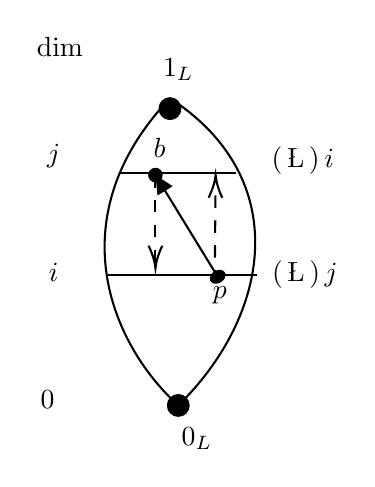
\begin{tikzpicture}[x=0.75pt,y=0.75pt,yscale=-1,xscale=1]
%uncomment if require: \path (0,300); %set diagram left start at 0, and has height of 300

%Curve Lines [id:da9559714668165431] 
\draw    (258,209.93) .. controls (225,179.93) and (200,118.93) .. (254,61.93) ;


%Curve Lines [id:da870462767582893] 
\draw    (258,209.93) .. controls (302,166.93) and (314,100.93) .. (254,61.93) ;


%Shape: Circle [id:dp6905850303089136] 
\draw  [fill={rgb, 255:red, 0; green, 0; blue, 0 }  ,fill opacity=1 ] (249,66.93) .. controls (249,64.17) and (251.24,61.93) .. (254,61.93) .. controls (256.76,61.93) and (259,64.17) .. (259,66.93) .. controls (259,69.69) and (256.76,71.93) .. (254,71.93) .. controls (251.24,71.93) and (249,69.69) .. (249,66.93) -- cycle ;
%Shape: Circle [id:dp3933822162001085] 
\draw  [fill={rgb, 255:red, 0; green, 0; blue, 0 }  ,fill opacity=1 ] (253,209.93) .. controls (253,207.17) and (255.24,204.93) .. (258,204.93) .. controls (260.76,204.93) and (263,207.17) .. (263,209.93) .. controls (263,212.69) and (260.76,214.93) .. (258,214.93) .. controls (255.24,214.93) and (253,212.69) .. (253,209.93) -- cycle ;
%Straight Lines [id:da2624167968218917] 
\draw    (230,97.93) -- (286,97.93) ;


%Straight Lines [id:da8790065247209863] 
\draw    (224,146.93) -- (296,146.93) ;


%Straight Lines [id:da09868631062113131] 
\draw    (248.04,100.64) -- (277,147.93) ;

\draw [shift={(247,98.93)}, rotate = 58.52] [fill={rgb, 255:red, 0; green, 0; blue, 0 }  ][line width=0.75]  [draw opacity=0] (8.93,-4.29) -- (0,0) -- (8.93,4.29) -- cycle    ;
%Shape: Circle [id:dp07389781898233405] 
\draw  [fill={rgb, 255:red, 0; green, 0; blue, 0 }  ,fill opacity=1 ] (244,98.93) .. controls (244,97.28) and (245.34,95.93) .. (247,95.93) .. controls (248.66,95.93) and (250,97.28) .. (250,98.93) .. controls (250,100.59) and (248.66,101.93) .. (247,101.93) .. controls (245.34,101.93) and (244,100.59) .. (244,98.93) -- cycle ;
%Shape: Circle [id:dp15699358050616063] 
\draw  [fill={rgb, 255:red, 0; green, 0; blue, 0 }  ,fill opacity=1 ] (274.03,147.49) .. controls (274.83,145.93) and (276.8,144.87) .. (278.43,145.11) .. controls (280.07,145.36) and (280.76,146.82) .. (279.97,148.38) .. controls (279.17,149.93) and (277.2,151) .. (275.57,150.75) .. controls (273.93,150.51) and (273.24,149.04) .. (274.03,147.49) -- cycle ;
%Straight Lines [id:da5019157895054271] 
\draw  [dash pattern={on 4.5pt off 4.5pt}]  (247,98.93) -- (247,141.93) ;
\draw [shift={(247,143.93)}, rotate = 270] [color={rgb, 255:red, 0; green, 0; blue, 0 }  ][line width=0.75]    (10.93,-3.29) .. controls (6.95,-1.4) and (3.31,-0.3) .. (0,0) .. controls (3.31,0.3) and (6.95,1.4) .. (10.93,3.29)   ;

%Straight Lines [id:da5990497530420301] 
\draw  [dash pattern={on 4.5pt off 4.5pt}]  (275.57,150.75) -- (275.98,100.93) ;
\draw [shift={(276,98.93)}, rotate = 450.48] [color={rgb, 255:red, 0; green, 0; blue, 0 }  ][line width=0.75]    (10.93,-3.29) .. controls (6.95,-1.4) and (3.31,-0.3) .. (0,0) .. controls (3.31,0.3) and (6.95,1.4) .. (10.93,3.29)   ;


% Text Node
\draw (201,37) node   {$\dim$};
% Text Node
\draw (258,48) node   {$1_{\mathbb{L}}$};
% Text Node
\draw (198,90) node   {$j$};
% Text Node
\draw (198,146) node   {$i$};
% Text Node
\draw (195,207) node   {$0$};
% Text Node
\draw (319,147) node   {$\begin{pmatrix}
	\L\\j
\end{pmatrix}$};
% Text Node
\draw (318,92) node   {$\begin{pmatrix}
	\L\\i
\end{pmatrix}$};
% Text Node
\draw (267,226) node   {$0_{\mathbb{L}}$};
% Text Node
\draw (249,86) node   {$b$};
% Text Node
\draw (278,157) node   {$p$};


\end{tikzpicture}

			%\caption{Desargues Konfiguration}
			%\label{Abb:natSpracheModellierung}
		\end{center}
\end{figure}

Seien $p\in\begin{pmatrix}
	\L\\
	i
\end{pmatrix}$ und $b\in\begin{pmatrix}
	\L\\
	j
\end{pmatrix}$.
Dann ist
\begin{align*}
	p I_{(i,j)}^\L&=\set{b\in'\begin{pmatrix}
		\L\\
		j
	\end{pmatrix}:p\leq_\L b'}\\
	I_{(i,j)}^\L b&=\set{p'\in\begin{pmatrix}
		\L\\
		i
	\end{pmatrix}:p'\leq_\L b}\\
	I_{(i,j)}^\L b&=\begin{pmatrix}
		\L(b)\\
		i
	\end{pmatrix}\mapsto
	\begin{pmatrix}
		\dim(b)\\
		i
	\end{pmatrix}_q=\begin{pmatrix}
		j\\
		i
	\end{pmatrix}_q
\end{align*}

\begin{satz}
	Es gilt weiter
	\begin{align*}
		pI^\L_{(i,j)}&=\set{b'\in\begin{pmatrix}
			\L\\
			j
		\end{pmatrix}:p\leq_\L b'}
		\overset{1-1}{\leftrightarrow}
		\set{b'/p\mid b'\in\begin{pmatrix}
			\L\\
			j
		\end{pmatrix}:p\leq_\L b}
		=\begin{pmatrix}
			\L(V/p)\\
			j-i
		\end{pmatrix}
		\mapsto\begin{pmatrix}
			n-i\\
			j-i
		\end{pmatrix}\\
		&\dim(b'/p)=\dim(b')-\dim(p)=j-i
	\end{align*}
	Ergebnis:
	\begin{align*}
		\Inz^\L_{(i,j)}
		=\klammern{
			\begin{pmatrix}
				\L\\
				i
			\end{pmatrix},
			\begin{pmatrix}
				\L\\
				j
			\end{pmatrix},
			I_{(i,j)}^\L
		}
	\end{align*}
	hat Parametertupel
	\begin{align*}
		\klammern{
			\begin{pmatrix}
				n\\
				i
			\end{pmatrix}_q,\begin{pmatrix}
				n-i\\
				j-i
			\end{pmatrix}_q,\begin{pmatrix}
				n\\
				j
			\end{pmatrix}_q,\begin{pmatrix}
				j\\
				i
			\end{pmatrix}_q
		}
	\end{align*}
\end{satz}

\begin{definition}
	Ist $f\colon\N\to\N_+$ eine Abbildung, so sei 
	\begin{align*}
		f!\colon\N\to\N_+,\qquad n\mapsto f(1)\mal f(2)\mal\ldots\mal f(n)
	\end{align*}
	Setze dann
	\begin{align*}
		\begin{pmatrix}
			n\\
			i
		\end{pmatrix}_f
		:=\frac{(f!)(n)}{(f!)(i)\mal(f!)(n-i)}
	\end{align*}
	Sonderfall: $(f!)(1)=f(1)$ und $(f!)(0)=1$
\end{definition}

\begin{satz}
	Dann gilt
	\begin{align*}
		\begin{pmatrix}
			n\\
			i
		\end{pmatrix}_f
		\mal\begin{pmatrix}
			n-i\\
			j-i
		\end{pmatrix}_f
		=\begin{pmatrix}
			n\\
			j
		\end{pmatrix}_f\mal\begin{pmatrix}
			j\\
			i
		\end{pmatrix}_f
	\end{align*}
	für beliebige $i,j\in\N$ mit $i\leq j\leq n$.
\end{satz}

\begin{beispiel}
	\begin{align*}
		f(n)&:=\#\set{t\in\L\big(\F^n_q\big)\mid\dim(t)1}\\
		f(1)&:=1\\
		\begin{pmatrix}
			n\\
			1
		\end{pmatrix}_f
		&=f(n)=\frac{q^n-1}{q-1}
	\end{align*}
\end{beispiel}

Wiederholung:
$V\simeq\F_q^n$, $\L=\L(V)=(L(V),\leq)$ Unterraumverband.
Hierbei ist "$\leq$" die Untervektorraum-Enthalten-Seins-Relation.
\begin{align*}
	L_i&:=\set{U\leq V\mid \dim(U)=i}
\end{align*}
Dann ist 
\begin{align*}
	\Inz_{i,j}^\L=\big(L_i,L_j,I_{i,j}\big)
	\qquad\mit\qquad
	I_{i,j}:=\set{(p,b)\in L_i\times L_j\mid p\leq b}
\end{align*}
taktische Konfiguration mit Parametertupel
\begin{align*}
	\klammern{
		\begin{pmatrix}
			n\\
			i
		\end{pmatrix}_q,\begin{pmatrix}
			n-i\\
			j-i
		\end{pmatrix}_q,\begin{pmatrix}
			n\\
			j
		\end{pmatrix}_q,\begin{pmatrix}
			j\\
			i
		\end{pmatrix}_q
	}
\end{align*}
wobei
\begin{align*}
	\begin{pmatrix}
		n\\
		1
	\end{pmatrix}_q
	=\frac{q^n-1}{q-1}
\end{align*}

\begin{bemerkungnr}
	$\begin{pmatrix}
		n\\
		i
	\end{pmatrix}_q$ heißt \define{Gauß-Koeffizient}
	\index{Gauß-Koeffizient}
	\begin{align*}
		\begin{pmatrix}
			n\\
			i
		\end{pmatrix}_q
		=\frac{
			\big(q^n-1\big)\mal\ldots\mal\big(q^{n-ii+1}-1\big)
		}{
			(q-1)\mal\ldots\mal\big(q^i-1\big)
		}
	\end{align*}
	Dies folgt aus
	\begin{align*}
		\begin{pmatrix}
			n\\
			i
		\end{pmatrix}_q\mal\begin{pmatrix}
			n-i\\
			j-i
		\end{pmatrix}_q
		=\begin{pmatrix}
			n\\
			j
		\end{pmatrix}_q\mal\begin{pmatrix}
			j\\
			i
		\end{pmatrix}_q
	\end{align*}
	und 
	\begin{align*}
		\begin{pmatrix}
			n\\
			1
		\end{pmatrix}_q=\frac{q^n-1}{q-1}
	\end{align*}
	
	Es gilt irgendwie auch:
	\begin{align*}
		\#V&=q^n\\
		\#\big(V\setminus\set{\vec{0}}\big)&=q^n-1\\
		\#\F_g v&=q\qquad\forall v\in V\setminus\set{\vec{0}}\\
		\#\big(\F_q\setminus\set{0}\big)v&=q-1\\
		\implies (q-1)\mal\begin{pmatrix}
			n\\
			1
		\end{pmatrix}_q&=q^n-1
	\end{align*}
\end{bemerkungnr}

\begin{bemerkungnr}
	Sei $f\colon\N\to\N_+$ Abbildung. 
	Setze
	\begin{align*}
		f!\colon\N\to\N_+,\qquad n\mapsto \prod\limits_{i\in[n]} f(i)=f(1)\mal f(2)\mal\ldots\mal f(n)
	\end{align*}
	Beachte $\prod\limits_{i\in\emptyset} f(i)=1$.
	Für $i,n\in\N$ sei
	\begin{align*}
		\begin{pmatrix}
			n\\
			i
		\end{pmatrix}_f
		:=\left\lbrace\begin{array}{cl}
			\frac{(f!)(n)}{(f!)(i)\mal(f!)(n-i)},&\falls i\leq n\\
			0, &\falls i>n
		\end{array}\right.
	\end{align*}
	Also ist 
	\begin{align*}
		\begin{pmatrix}
			n\\
			i
		\end{pmatrix}_f
		=\frac{
			f(n)\mal\ldots\mal f(n-i+1)
		}{
			f(1)\mal\ldots\mal f(i)
		}\qquad\forall i\leq n
	\end{align*}
	Für eine Abbildung
	\begin{align*}
		[~]\colon\N\times\N\to\N,\qquad
		(i,n)\mapsto\begin{bmatrix}
			n\\
			i
		\end{bmatrix}\\
		\mit~
		\supp([~])
		\overset{\Def}{=}
		\set{(i,n)\in\N\times\N\mid i\leq n}
		=\set{(i,n)\in\N\times\N\mid i\leq n}
	\end{align*}
	 Link: \url{https://de.wikipedia.org/wiki/Inzidenzalgebra}
	 Es gilt stets:
	 \begin{align}\label{eq:24.4Stern}\tag{$*$}
	 	\begin{bmatrix}
	 		n\\
	 		i
	 	\end{bmatrix}\mal\begin{bmatrix}
	 		n-i\\
	 		j-i
	 	\end{bmatrix}
	 	=\begin{bmatrix}
	 		n\\
	 		j
	 	\end{bmatrix}\mal\begin{bmatrix}
	 		j\\
	 		i
	 	\end{bmatrix}
	 	\qquad\forall i\leq j\leq n
	 \end{align}
	 Das heißt
	 \begin{align*}
	 	\klammern{
			\begin{bmatrix}
				n\\
				i
			\end{bmatrix},
			\begin{bmatrix}
				n-i\\
				j-i
			\end{bmatrix};\begin{pmatrix}
				n\\
				j
			\end{pmatrix},\begin{bmatrix}
				j\\
				i
			\end{bmatrix}
	 	}
	 \end{align*}
	 ist formales taktisches Konfigurationsquadrupel.
\end{bemerkungnr}

Ist umgekehrt $[~]\colon\leq_\N\to\N_+$ mit \eqref{eq:24.4Stern} gegeben, so ist $[~]=(~)_f$ für
\begin{align*}
	f\colon\N\to\N_+,\qquad n\mapsto\begin{bmatrix}
		n\\
		1
	\end{bmatrix}
\end{align*}
Folglich ist $f(1)=1$.

\begin{bemerkungnr}\
	\begin{enumerate}[label=(\arabic*)]
		\item Warnung! Gegenbeispiel:
	$[~]\colon\leq_\N\to\N_+,~(i,n)\mapsto 2$ erfüllt \eqref{eq:24.4Stern}, aber es existiert \betone{kein} $f\colon\N\to\N_+$ mit $[~]=(~)_f$.
		\item $[~]\colon\leq_\N\to\N_+,~(i,n)\mapsto1$ erfüllt $[~]=(~)_f$ für $f\colon\N\to\N_+,~ n\mapsto 1$.
		\item \eqref{eq:24.4Stern} ist ein Beispiel einer Funktionalgleichung.
	\end{enumerate}
\end{bemerkungnr}

\begin{beispiel}
	Weitere "interessanter" taktischer Konfigurationen via freier endlichen Ring Moduln.\nl
	Sei $\S=\big(S,+,\mal,0,1\big)$ ein \define{Semiring (mit Eins)}, d.h. $\S_{\add}:=\big(S,+,\mal\big)$ ist kommutatives Monoid und $\S_{\mult}:=\big(S,\mal,1\big)$ ist Monoid derart, dass das Distributivgesetz
	\index{Semiring}
	\begin{align*}
		a\mal(b+c)=(a\mal b)+(a\mal c)=:a\mal b+a\mal c\qquad\forall a,b,c\in S
	\end{align*}
	gilt.
	Sind $\S=\big(S,+,\mal,0,1\big)$ und $\S'=\big(S',+',\mal',0',1'\big)$ Semiringe, so heiße eine Abbildung $\varphi\colon S\to S'$ \define{Morphismus}, falls $\varphi$ Morphismus von $\S_{\add}$ nach $\S'_{\add}$ und $\varphi$ Morphismus von $\S_{\mult}$ nach $\S_{\mult}'$ bildet, d.h. es gilt für alle $a,b\in S$:
	\index{Morphismis}
	\begin{enumerate}
		\item $\begin{aligned}
			\varphi(a+b)&=\varphi(a)+'\varphi(b)
		\end{aligned}$
		\item $\begin{aligned}
			\varphi(a\mal b)=\varphi(a)\mal'\varphi(b)
		\end{aligned}$
		\item $\begin{aligned}
			a\mal 0=0=0\mal a
		\end{aligned}$
		\item $\begin{aligned}
			1\neq 0
		\end{aligned}$
		\item $\begin{aligned}
			\varphi(1)=1'
		\end{aligned}$
	\end{enumerate}
	
	Ist $\M=(M,+\vec{0)})$ kommutativer Monoid und $\S=(S,+,\mal,0,1)$ Semiring (SR), so heiße 
	\index{Sclaling}
	\begin{align*}
		\scal\colon S\to\End(\M)
	\end{align*}
	ein \define{Scaling}, falls
	\begin{align*}
		\End(\M):=\big(\End(M),+,\mal,0,\id_M\big)
	\end{align*}
	Endomorphismen-Semiring von $\M$.\\
	$\scal$ Morphismus von $\S$ nach $\End(\M)$.\nl
	Die Abbildung $S\times M\to M,~(s,m)\mapsto sm:=\big(\scal(s)\big)m$
	heiße das zugehörige \define{Skalarprodukt}.
	\index{Skalarprodukt}\\
	Wir nennen dann $(\M,\S,\scal)$ einen \define{Semiring-Modul} bzw. sagen $\M$ bildet (bzgl. $\scal$) einen Modul über $\S$.
	\index{Semiring-Modul}
\end{beispiel}

\begin{bemerkungnr}
	Sei $\F_q$ endlicher Körper ($q$-elementig) und sei $V$ $n$-dimensionaler Vektorraum über $\F_q$ ($n\in\N_+$).
	Für $i,j\in\N$ mit $i\leq j\leq n$ und $\L:=\L(V)$ Unterraumverband von $V$ ist dann
	\begin{align*}
		\Inz_{(i,j)}^\L&:=\big(L_i,L_j,I_{i,j}\big)\mit\\
		L_i&:=\set{p\leq V\mid\dim(p)=i}
		\und \\
		L_j&:=\set{b\leq V\mid\dim(b)=j}
		\und\\
		I_{i,j}&:=\set{(p,b)\in L_i\times L_j\mid p\leq b}
	\end{align*}
	eine taktische Konfiguration mit Parametertupel
	\begin{align*}
		\klammern{
			\begin{pmatrix}
				n\\
				i
			\end{pmatrix}_q,
			\begin{pmatrix}
				n-i\\
				j-i
			\end{pmatrix}_q;
			\begin{pmatrix}
				n\\
				j
			\end{pmatrix}_q,
			\begin{pmatrix}
				j\\
				i
			\end{pmatrix}_q
		}
	\end{align*} wobei $\begin{pmatrix}
		n\\
		i
	\end{pmatrix}_q:=\begin{pmatrix}
		n\\
		i
	\end{pmatrix}_f$ für $f\colon\N\to\N_+,~i\mapsto q^i-1$ gerader der Gaußkoeffizient zu $n$ über $i$ bzgl. $q$ ist.
	Gilt $0<i<j<n$, so ist
	\begin{align*}
		\Aut\big(\Inz_{i,j}^\L\big)\cong\PGL_n(\F_q)
	\end{align*}
	(ohne Beweis). Auf der linken Seite steht die projektive lineare Gruppe von $\F_q^n$.
	\begin{align*}
		f!\colon\N\to\N_+,\qquad n\mapsto\prod\limits_{i\in[n]} f(i)\\
		\begin{pmatrix}
			n\\
			i
		\end{pmatrix}_f:=\frac{(f!)(n)}{(f!)(i)\mal (f!)(n-i)}\qquad\forall 0\leq i\leq n
	\end{align*}
	Die Abbildung $[~]\colon\leq_\N\to\N_+$ erfüllt
	\begin{align*}
		\begin{bmatrix}
			n\\
			i
		\end{bmatrix}\mal
		\begin{bmatrix}
			n-i\\
			j-i
		\end{bmatrix}=\begin{bmatrix}
			n\\
			j
		\end{bmatrix}\mal
		\begin{bmatrix}
			j\\
			i
		\end{bmatrix}\qquad\forall i,j,n\in\mit i\leq j\leq n
	\end{align*}
	Und $\begin{bmatrix}
		1\\
		1
	\end{bmatrix}=1$ genau dann, wenn $[~]=(~)_f$ für $f\colon\N\to\N_+,~n\mapsto\begin{bmatrix}
		n\\
		1
	\end{bmatrix}$
\end{bemerkungnr}

\textbf{Frage:} Lässt sich obiges auf endliche freie Ring-Moduln ausweiten?

\subsection{Ausflug: Semiring-Moduln (Semimodule)}
Sei $\S=(S,+,\mal,0,1)$ ein Semiring ($\S_{\add}$ kommutatives Monoid und $\S_{\mult}$ Monoid)
Es gilt also:
\begin{enumerate}
	\item $a\mal(b+c)=(a\mal b)+(a\mal c)=:a\mal c+b\mal c$ Distributivgesetz
	\item $(a+b)\mal c=a\mal c+b\mal c$ Distributivgesetz
	\item $0\mal a=0=a\mal 0$ Nullabsorption
	\item $a\neq 0$ Reichhaltigkeit
\end{enumerate}

\begin{beispiel}\
	\begin{itemize}
		\item Boolscher Semiring: $\big(\set{0,1},+,\mal,0,1\big)$ mit $1+1=1$
		\item $\ul{\N}=\big(\N,+,\mal,0,1\big)$ ist der natürliche Semiring
		\item $\F_2=\big(\set{0,1},+,\mal,0,1\big)$ mit $1+1=0$
		\item Ringe, Körper $\Z,\Q,\R,\C$
		\item \define{tropischer Semiring} $\big([0,\infty],\min,+,\infty,0\big)$
	\end{itemize}
\end{beispiel}

\begin{definition}
	Seien $\S=(S,+,\mal,0,1)$ und $\S'=(S',+',\mal',0',1')$ Semiringe.
	Eine Abbildung $\varphi\colon S\to S'$ heißt \define{Morphismus} von $\S$ nach $\S'$, falls $\varphi$ Morphismus von $\S_{\add}$ nach $\S_{\add}'$ und $\varphi$ Morphismus von $\S_{\mult}$ nach $\S_{\mult}'$.\nl
	Ein bijektiver Morphismus heißt \define{Isomorphismus}.
	Ein Morphismus in sich heißt \define{Endomorphismus}.


\begin{itemize}
	\item $\S$ \define{Ring}: $\S$ Semiring und $\S_{\add}$ Gruppe
	\item $\S$ \define{Divisionsring / Schiefkörper:} $\S$ Ring und $\S_{\mult}^\times=\big(S\setminus\set{0},\mal,1\big)$ Gruppe
	\item $\S$ \define{Körper}: $\S$ Divisionsring und $\S_{\mult}$ kommutativ
\end{itemize}

\end{definition}

Ist $\M=(M,+,\vec{0})$ kommutatives Monoid, so ist $\End(M)$ Menge der Endomorphismen von $\M$ d.h. $\varphi\colon M\to M$ Abbildung mit
\begin{align*}
	\varphi(x+y)=\varphi(x)+\varphi(y)\qquad\forall x,y\in M
\end{align*}
und $\varphi(\vec{0})=\vec{0}$.
Dann ist 
\begin{align*}
	\End(\M):=\big(\End(M),+,\circ,0,\id_M\big)
\end{align*}
wobei $\circ$ die Abbildungsverkettung ist und
	\begin{align*}
		\varphi+\psi\colon:M\to M,\qquad x\mapsto \varphi(x)+\psi(x)\qquad\forall \varphi,\psi\in\End(M)\\
		0\colon M\to M,\qquad x\mapsto\vec{0}
	\end{align*}
	ein Semiring, der sogenannte \define{Endomorphismen-Semiring zu $\M$}.
	
\begin{lemma}
	Ist $\M$ kommutative Gruppe, so ist $\End(\M)$ ein Ring.
\end{lemma}

\subsubsection{Lineare Algebra über Semiring-Moduln}
Sei $\S=(S,+,\mal,0,1)$ Semiring ("abstrakte Skalare", skalarer Bereich) und $\M=(M,+,\vec{0})$ kommutatives Monoid ("abstrakte Vektoren", vektorieller Bereich) und sei $\scal\colon\End(\M)$ Morphismus, genannt \define{Scaling}.
\index{Scaling}
Dann nennen wir $\mathcal{M}:=(\M,\S,\scal)$ auch \define{Semiring-Modul}.
\index{Semiring-Modul}
Es wird durch $\mathcal{M}$ ein \define{skalare Multiplikation}
\index{skalare Multiplikation}
\begin{align*}
	S\times M\to M,\qquad (s,m)\mapsto s\mal m:=\big(\scal(s)\big) m
\end{align*}
induziert. Dies ist die \define{kontravariante Sicht}.\index{kontravariante Sicht}\\
\define{Kovariante Sicht:}\index{kovariante Sicht}
\begin{align*}
	M\times S\to M,\qquad (m,s)\mapsto m\mal s:=m(s-\scal)
\end{align*}
wobei $s-\scal$ das zu $s\in S$ gehörige $s$-Scaling sei, d.h. $s-\scal:=\scal(s)$.\\
Für $\mathcal{M}$ schreiben wir auch $\S^\M$ oder sagen $\M$ ist Semiring über $\S$ via $\scal$.\\
(Kovariante bzw. Kontravariante Sicht ist nur eine Frage der Notation)

\begin{beispiel}[Freie Semiring-Moduln]\enter
	Sei $\S=(S,+,\mal,0,1)$ Semiring und sei $N$ eine Menge.
	Dann sei
	\begin{align*}
		\Mod(\S,N):=\klammern{\S_{\add}^{(N)},\S,\scal}
		\mit
		\S_{\add}^{(N)}:=\set{u\in S^N\mid\supp(u)\text{ endlich}}
		\mit\\
		\supp(u):=\set{i\in N\mid u(i)\neq 0}
		u+w\colon N\to S,\qquad i\mapsto u(i)+w(i)
		\vec{0}\colon N\to S,\qquad i\mapsto 0
	\end{align*}
	$\scal\colon S\to\End\klammern{\S_{\add}^{(N)}}$ via jedes $s\in S$ erfüllt $\scal(s)\colon S^{(N)}\to S^{(N)},~u\mapsto s\mal u:=(s\mal u(i))_{i\in\N}$, d.h. $s\mal u\colon N\to S,~i\mapsto s\mal u(i)$.
	ein Semiring-Modul, der sogenannte $N$-freie Semiring-Modul über $\S$.
\end{beispiel}

\subsection{(linksseitiger) Semiring-Modul}
$\mathcal{M}=(\M,\S,\scal)$\\
$\M=(M,+,\sigma)$ vektorieller Bereich\\
$\S=(S,+,\mal,0,1)$ skalarere Bereich (Semiring)\\
$\scal\colon\S\to\End(\M)$ Scaling (Morphismus)\\
rechtsseitiger Semiring-Modul:\\
$\scal\colon\S\to\End_{\cov}(\M)$ \define{kovariantes Scaling}\\
skalare Multiplikation:
\begin{align*}
	S\times M\to M,\qquad(s,m)\mapsto s m:=\scal(s)m
\end{align*}

\begin{beispiel}
	\begin{align*}
		\Mod(\S,N)&:=\klammern{\S_{\add}^{(N)},\S,\scal}
	\end{align*}
	wobei $N$ eine Menge und $\S=(S,+,\mal,0,1)$ ein Semiring ist.
	Außerdem: ist
	\begin{align*}
		\S_{\add}^{(N)}:=\klammern{S^{(N)},+,\vec{0}}
	\end{align*}
	die \define{$N$-fache Copotenz von $\S_{\add}$}.
	\begin{align*}
		S^{(N)}:=\set{ u\in S^N\mid\supp(u)\text{ endlich}}\\
		u+w\colon N\to S,\qquad i\mapsto u(i)+w(i)\qquad\forall u,w\in S^{(N)}
	\end{align*}
	und
	\begin{align*}
		\sigma\colon N\to S,\qquad i\mapsto 0
	\end{align*}
	sowie
	\begin{align*}
		\scal\colon S\to\End\klammern{\S_{\add}^{(N)}},\qquad s\mapsto \lambda_s
	\end{align*}
	wobei
	\begin{align*}
		\lambda_s\colon S^{(N)}\to S^{(N)},\qquad
		u\mapsto su:=\klammern{s\mal u(i)}_{i\in N}
	\end{align*}
	
	$\Mod(\S,N)$ heiße der \define{$N$-freie Standardmodul} über $\S$.
	Dann heiße
	\begin{align*}
		\delta^N&\colon N\to S^{(N)},\qquad i\mapsto\delta_i^N\qquad\text{wobei}\\
		 \delta_i^N&\colon N\to S,\qquad j\mapsto\left\lbrace\begin{array}{cl}
		 	1, &\falls j=1\\
		 	0, & \sonst
		 \end{array}\right.
	\end{align*}
	die \define{Standardbasis} von $\Mod(\S,N)$ (bzgl. $(\S,N)$ ist.
\end{beispiel}

\subsection{Was ist eine Linearkombination?}
Sei $\mathcal{M}=\klammern{\M,\S,\scal}$ Semiring-Modul und sei $N$ eine Menge.
Für $n\in S^{(N)}$ und $\gamma\in M^N$ heiße dann
\index{Linearkombination}
\begin{align*}
	u*\gamma:=\sum\limits_{i\in N} u(i)\mal\gamma(i):=\sum\limits_{i\in\supp(u)} u(i)\mal\gamma(i)\in M
\end{align*}
die \define{Linearkombination} von $u$ mit $\gamma$ in $\mathcal{M}$.
$u$ heißt \define{Koeffizientenfamilie} und $\gamma$ \define{Vektorenfamilie}
\index{Koeffizientenfamilie}
\index{Vektorenfamilie}

\subsubsection{Linearkombinationsabbildung}
Sei $\mathcal{M}=(\M,\S,\scal)$ Semring-Modul und sei $N$ Menge und $\gamma\in M^N$, d.h. $\gamma=:\big(\gamma(i)\big)_{i\in N}$ Vektorenfamilie in $\mathcal{M}$.
Dann heiße
\begin{align*}
	f_\gamma\colon S^{(N)}\to M,\qquad
	u\mapsto u*\gamma
\end{align*}
die \define{Linearkombinationsabbildung} zu $\gamma$ bzgl. $\mathcal{M}$.
\index{Linearkombinationsabbildung}

\begin{satz}
	Es gilt
	\begin{align*}
		&f_\gamma\circ\delta^N=\gamma\\
		&\begin{tikzcd}[ampersand replacement=\&]
                               \& N \arrow[rd, "\gamma"] \arrow[ld, "\delta^N"'] \&   \\
S^{(N)} \arrow[rr, "f\gamma"'] \&                                                \& M
\end{tikzcd}
	\end{align*}
\end{satz}

\begin{erinnerung}
	Seien $V,W$ Vektorräume über Körper $K$.
	\begin{enumerate}
		\item Klassische Situation: Ist $f\colon V\to W$ linear Abbildung, so ist
		\begin{align*}
			\Kern(f):=\set{v\in V\mid f(v)=0_W}
		\end{align*}
		der \define{große Kern}. 
		Dieser ist Untervektorraum von $V$.
		\index{großer Kern}
		\item Allgemeine Situation:
		Sind $A,B$ Mengen und ist $f\colon A\to B$ Abbildung, so ist
		\begin{align*}
			\ker(f):=\set{(a,c)\in A\times S\mid f(a)=f(c)}
		\end{align*}
		der \define{kleine Kern.}
		Dies ist eine Äquivalenzrelation auf $A$.
		\index{kleiner Kern}
		\item Es gilt:
		\begin{align*}
			\Kern(f)=0_V \ker(f)=:[0_V]\ker(f)
		\end{align*}
	\end{enumerate}
\end{erinnerung}

\begin{definition}\
	\begin{itemize}
		\item $\gamma$ \define{unabhängig} (bzgl. $\mathcal{M}$)
		$
			\defiff f_\gamma \text{ injektiv}
			\iff \ker(f_\gamma)=\triangle_{S^{(N)}}
		$
		\item $\gamma$  \define{erzeugend} (bzgl. $\mathcal{M}$) $\defiff f_\gamma$ surjektiv
		\item $\gamma$ \define{Basis} von $\mathcal{M}\defiff f_\gamma$ bijektiv
	\end{itemize}
\end{definition}

\begin{beispiel}[Standardbasis ist eine Basis]\enter
	$\delta^N$ ist Basis von $\Mod\klammern{\S,N}$.
	Begründung: $f_{\delta^N}=\id_{S^{(N)}}$
\end{beispiel}

\subsection{Semring-Modul Fortsetzung}

\begin{proposition}
	Sei $\mathcal{M}=\klammern{\M,\S,\scal}$ Semiring-Modul und seien $K$ und $N$ Mengen.
	Ferner seien $\chi\in K^N$ und $\lambda\in M^K$ sowie $\gamma\in M^N$ mit
	\begin{align*}
		\lambda=\gamma\circ\chi\qquad f_\lambda\circ\delta^K\qquad
		f_\gamma\circ\delta^N=\gamma\\
		\begin{tikzcd}[ampersand replacement=\&]
			\& K \arrow[ld, "\delta^K"'] \arrow[rd, "\lambda"] \arrow[rr, "\chi"] \&   \& N \arrow[rd, "\delta^N"] \arrow[ld, "\gamma"'] \&                                \\
			S^{(K)} \arrow[rr, "f_\lambda"'] \& \& M \&                                                \& S^{(N)} \arrow[ll, "f_\gamma"]
		\end{tikzcd}
	\end{align*}

	\begin{enumerate}[label=(\arabic*)]
		\item Ist $\lambda$ erzeugend bzgl. $\mathcal{M}$, so ist auch $\gamma$ erzeugend bzgl. $\mathcal{M}$.
		\label{item:prop1}
	\end{enumerate}
\end{proposition}

\begin{proof}
	\betone{Zeige \ref{item:prop1}:}\\
	Da $\lambda$ erzeugend ist, existiert zu jedem $m\in M$ ein $v\in S^{(K)}$ mit
	\begin{align*}
		v*\lambda=f_\lambda(v)=m
	\end{align*}
	Für 
	\begin{align*}
		u\colon N\to S,\qquad
		i\mapsto\sum\limits_{k\in\chi^{-1}(i)} vk
	\end{align*}
	gilt dann
	\begin{align*}
		f_\gamma(u)
		&=u*\gamma\\
		&=\sum\limits_{i\in N} u(i)\gamma(i)\\
		&=\sum\limits_{i\in N}\klammern{\sum\limits_{k\in\chi^{-1}(i)} v(k)}\gamma(i)\\
		&=\sum\limits_{i\in N}\sum\limits_{k\in\chi^{-1}(i)} v(k)\gamma(i)\\
		\overset{\chi(k)=1}&{=}
		\sum\limits_{i\in N}\sum\limits_{k\in\chi^{-1}(i)} v(k)\gamma(\chi(k))\\
		&=\sum\limits_{k\in K} v(k)\gamma(\chi(k))\\
		&=v*\lambda\\
		&=m
	\end{align*}
	Also ist auch $f_\gamma$ surjektiv, d.h. $\gamma$ ist erzeugend.\nl
\end{proof}

\begin{notation}
	Ist $f\colon A\to B$ Abbildung so sei
	\begin{align*}
		f^-\colon B\to\Potenzmenge{A},\qquad
		b\mapsto\set{a\in A\mid f(a)=b}
	\end{align*}
\end{notation}

\betone{Fragen:}
\begin{enumerate}
	\item Was passiert, wenn $\chi$ injektiv ist?
	\item Was passiert, wenn $\chi$ surjektiv ist?
\end{enumerate}

\betone{Vorbetrachtung:}\\
Für jedes $v\in S^{(K)}$ erfüllt
\begin{align*}
	u\colon N\to S,\qquad
	i\mapsto\sum\limits_{k\in\chi^-(i)}v(h)
\end{align*}
die Gleichung
\begin{align}\label{eq080519}\tag{$*$}
	f_\gamma(v_\chi)=v_\chi*\gamma=v*\lambda=f_\lambda(v)
\end{align}

Zu (a): Sei $\chi$ injektiv.
Für jedes $v\in S^{(K)}$ und $i\in N$ ist
\begin{align*}
	v_\chi(i)=\left\lbrace\begin{array}{cl}
		v_k, &\falls \exists k\in K:\chi(k)=i,\text{ d.h. }\chi^{-}(i)=\set{k}\\
		0, &\sonst (\chi^{-}(i)=\emptyset
	\end{array}\right.
\end{align*}
Also ist $v_\chi\circ\chi=v$, da $v_\chi(\chi_k)=v(k)$ für jedes $k\in K$.
Angenommen $\gamma$ ist unbhängig bzgl. $\mathcal{M}$.
Dann ist auch $\lambda$ unabhängig bzgl. $\mathcal{M}$.\nl
\betone{Ergebnis zu (a):} Ist $\chi$ injektiv und $\gamma$ unabhängig bzgl. $\mathcal{M}$, so ist auch $\lambda=\gamma\circ\chi$ unabhängig bzgl. $\mathcal{M}$.\nl
\betone{Zu (b):} Mit dem Auswahlaxiom erhält man dann eine Abbildung $\eta\colon N\to K$ mit $\chi\circ\gamma=\id_N$.\\
\betone{Beobachtung:} Aus $\lambda=\gamma\circ\chi$ folgt dann
\begin{align*}
	\lambda\circ\eta
	=\klammern{\gamma\circ\chi}\circ\eta
	=\gamma\circ\underbrace{\klammern{\chi\circ\eta}}_{=\id_N}=\gamma
\end{align*}
Mit (1) folgt nunmehr:\\
Ergebnis (3): Ist $\chi$ surjektiv und ist $\gamma$ erzeugend bzgl. $\mathcal{M}$, so folgt mit dem Auswahlaxiom, dass auch 
$\lambda=\gamma\circ\chi$ erzeugend. bzgl. $\mathcal{M}$ ist.\nl
(4) Anwendunggen:
\begin{itemize}
	\item Mit dem Auswahlaxiom gilt:\\
Ist $\chi$ surjektiv, so ist $\gamma$ erzeugt genau dann, wenn $\lambda$ erzeugt ist.
	\item Warnung: Ist $\chi$ injektiv und $\lambda$ unabhängig, so kann es sein, dass $\gamma$ nicht unabhängig ist:
\begin{beispiel}
	$K=[1]$, $N=[2]$, $\gamma\colon N\to S,~i\mapsto 1$ nicht unabhängig bzgl. $\Mod(\S,K)$ aber $\lambda\colon[1]\to S,~1\mapsto 1$ ($f_\lambda=\id_{S^K}$ bzgl. $\mod(\S,K)$ obwohl $\lambda=\gamma\circ\chi$ ist für $\chi\colon K\to N,~1\mapsto 1$.
	\end{beispiel}
	\item Ist $\chi$ bijektiv (dann ist $\chi^{-1}$ bijektiv und es gilt $\gamma=\lambda\circ\chi^{-1}$, so ist $\gamma$ Basis von $\mathcal{M}$ genau dann, wenn $\lambda$ Basis von $\mathcal{M}$ ist.
\end{itemize}



